

\author[Niklas Brunn]{Nix}


\beamertemplatenavigationsymbolsempty{}

\logo{
\includegraphics[height=1cm]{Bilder/logo}}



\section{ODE$^{2}$VAE}

\begin{frame}
    \frametitle{ODE$^{2}$VAE}
    Wir wollen als nächstes \emph{time series} mit einen \emph{ODE$^{2}$VAE} modellieren\\ 
    \text{ }\\
    \text{ }
    \begin{itemize}
    	\item[ ] \emph{ODE$^{\ 2}$VAE: Deep generative second order ODEs with Bayesian neural networks} von Ç. Yıldız, M. Heinonen und H. Lähdesmäki
    \end{itemize}	
\end{frame}




\begin{frame}
	\frametitle{Idee}
	\begin{itemize}
	\item Bewegungen (z.B. Fadenpendel) lassen sich nicht gut mit einem Standard-VAE modellieren\\
	\item \textbf{neuer Ansatz:} Zeitliche Abhängigkeit der Daten berücksichtigen und die Bewegung durch Differentialgleichungen zweiter Ordnung (ODE$^{2}$) modellieren 
	\item \textbf{Vorteile:} Wir können so zu beliebigen Zeitpunkten abfragen und auch Prognosen für die Zukunft generieren
	\end{itemize}
\end{frame}



\begin{frame}
    \frametitle{Notation}
    \begin{itemize}
    	\item \textbf{Gegeben:} \emph{time series} $\mathbf{x}_{0:T}=(\mathbf x_{0}, \mathbf x_{1}, \ldots,\mathbf x_{T})\in \mathbb{R}^{D\times T}$ zu beobachteten Zeitpunkten $t_{0}, t_{1},\ldots,t_{T}$\\
    	\item \textbf{Annahme:} Zeitliche Änderung der latenten Darstellung kann stetig durch eine ODE$^{2}$ beschrieben werden\\
    	\item Zugehörigen latenten Zustände zu den beobachteten Zeitpunkten sind $\mathbf z_{0:T}=(\mathbf z_{0}, \mathbf z_{1}, \ldots, \mathbf z_{T})\in \mathbb{R}^{d\times T}$\\ 
    	\item Latente Zustände werden in Positions- und Geschwindigkeitskomponente aufgeteilt $\mathbf z_{t}=(\mathbf s_{t}, \mathbf v_{t})$
    \end{itemize}
\end{frame}




\begin{frame}
\frametitle{Notation}
    \begin{itemize}
    	\item Die ODE$^{2}$ lässt sich als ein System zweier ODE$^{1}$ schreiben
    \end{itemize}	
    {\footnotesize\begin{align*}
	    \dfrac{\partial^2 \mathbf{z}(t)}{\partial^2 t}=f_{\boldsymbol{\psi}}\left(\mathbf{z}(t), \tfrac{\partial \mathbf{z}(t)}{\partial t}, t\right)%, \\
	    %&\begin{cases*}
	    %\tfrac{\partial \mathbf{s}(t)}{\partial t}=\mathbf v(t) \\
	    %\tfrac{\partial \mathbf{v}(t)}{\partial t}=f_{\boldsymbol{\psi}}(\mathbf s(t), \mathbf v(t), t) \\
	    %\end{cases*}
	\end{align*}}
    \begin{itemize}
    	\item $f_{\boldsymbol{\psi}}$ ist dabei ein NN, welches das Beschleunigunsfeld erlernt
    	\item Lösen des Anfangswertproblems in $\mathbf{z}_{0}=(\mathbf{s}_{0}, \mathbf{v}_{0})$ liefert zu beliebigen Zeitpunkten $T$ eine Lösung
	\end{itemize}
    {\footnotesize\begin{align*}
    \left(\begin{array}{cc}
    \mathbf s_{T} \\
    \mathbf v_{T}
    \end{array}\right)
    =
    \left(\begin{array}{cc}
    \mathbf s_{0} \\
    \mathbf v_{0}
    \end{array}\right)
    +
    \int_{0}^{T}
    \left(\begin{array}{cc}
    \mathbf v(t) \\
    f_{\boldsymbol{\psi}}(\mathbf s(t), \mathbf v(t), t)
    \end{array}\right)
    \mathrm{d}t.
    \end{align*}}
\end{frame}




\begin{frame}
\frametitle{Modell}
Das Modell besteht aus den folgenden Komponenten:
\begin{itemize}
	\item Als \textbf{Prior} für die latente Ausgangsposition $p(\mathbf{s}_{0})$ und die latente Ausgangsgeschwindigkeit $p(\mathbf{v}_{0})$ wird eine Standardnormalverteilung gewählt
	\item Einem \textbf{Position-Encoder} welcher mit $\mathbf{x}_{0}$ die erste latente Ausgangsposition $\mathbf{s}_{0}$ encodiert und einem \textbf{Velocity-Encoder} welcher mit den ersten $m\geq2$ Werten $\mathbf{x}_{m}$ die latente Ausgangsgeschwindigkeit encodiert\\
    \item Einem \textbf{ODE-Netzwerk} welches zu einem Anfangswert eine Kurve im latenten Raum bestimmt\\
    \item Einem \textbf{Decoder}, welcher die aus der Kurve resultierenden latenten Positionen decodiert
\end{itemize}
\end{frame}




\begin{frame}
    \frametitle{Modell}
    	\begin{figure}[h!]
    	\centering
    	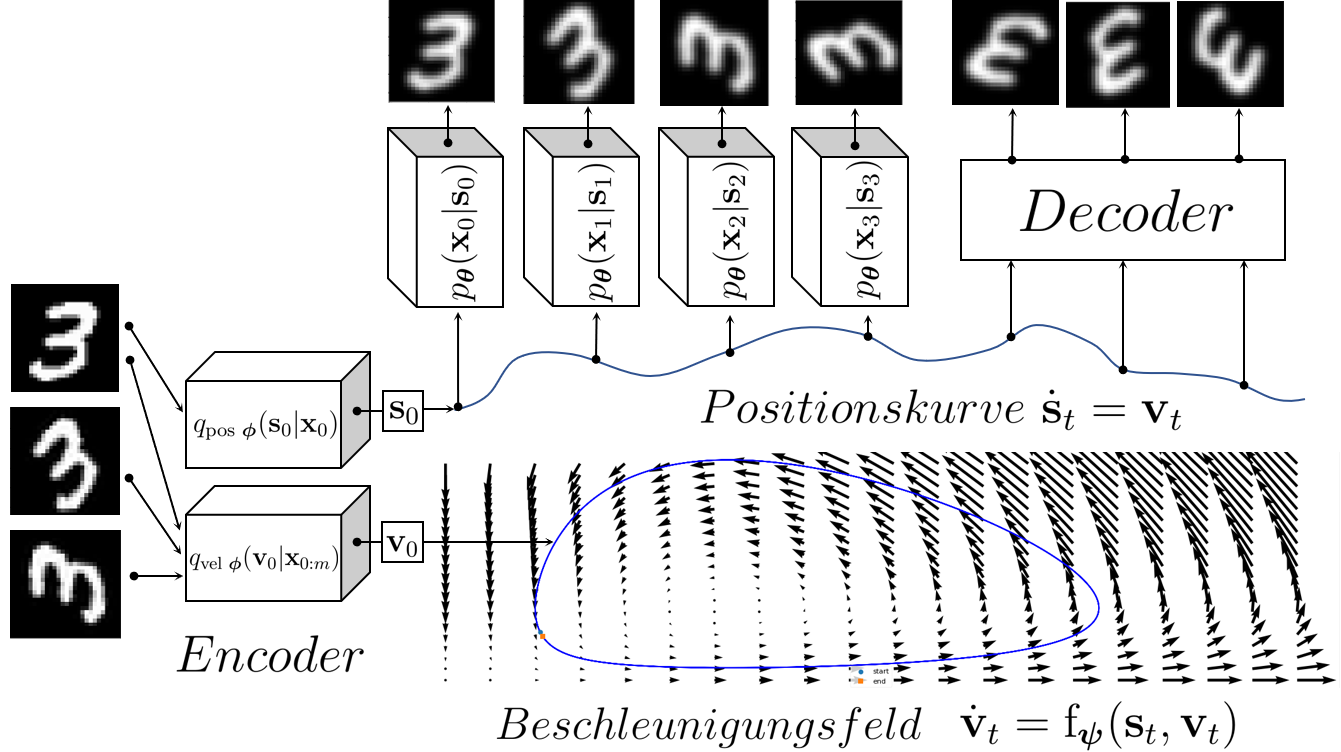
\includegraphics[scale=0.36]{Bilder/ODE2VAE_ODE_Net}
    \end{figure}
\end{frame}




\begin{frame}
    \frametitle{Training}
    Als Trainingskriterium verwenden wir erneut die \textbf{ELBO} 	
    	{\footnotesize\begin{align*}
            \log\big(p_{\boldsymbol{\theta}}(\mathbf{x}_{0:T})\big)&\ge \E_{\mathbf{z}_{0:T}\sim q_{\boldsymbol\phi,\boldsymbol\psi}}
            \left[\log\big(p_{\boldsymbol\theta}\left(\mathbf{x}_{0:T}|\mathbf{z}_{0:T}\right)\big)\right] - D_{KL}\big[q_{\boldsymbol\phi,\boldsymbol\psi}(\mathbf{z}_{0:T}|\mathbf{x}_{0:m})||p_{\boldsymbol\theta,\boldsymbol\psi}(\mathbf{z}_{0:T})\big]\\
            &=\underbrace{\E_{\mathbf{z}_{0}\sim q_{\text{enc }\boldsymbol\phi}}
    	    \left[\log\big(p_{\boldsymbol\theta}\left(\mathbf{x}_{0}|\mathbf{z}_{0}\right)\big)\right] - D_{KL}\big[q_{\text{enc }\boldsymbol\phi}(\mathbf{z}_{0}|\mathbf{x}_{0:m})||p_{\boldsymbol\theta}(\mathbf{z}_{0})\big]}_{\text{Vanilla-VAE ELBO}}\\ &+ \underbrace{\sum_{t=1}^T \E_{\mathbf{z}_{t}\sim q_{\text{ode }\boldsymbol\psi}}
    	    \left[\log\big(p_{\boldsymbol\theta}\left(\mathbf{x}_{t}|\mathbf{z}_{t}\right)\big)\right] - D_{KL}\big[q_{\text{ode }\boldsymbol\psi}(\mathbf{z}_{t}|\mathbf{x}_{0:m})||p_{\boldsymbol\theta,\boldsymbol\psi}(\mathbf{z}_{t})\big]}_{\text{dynamic loss}}
    \end{align*}}
    Während des Trainings sieht das Modell die gesamte \emph{time series}
\end{frame}


\begin{frame}
    \frametitle{Ergebnisse}
    \emph{bouncing Balls}
    \begin{figure}[!htbp]
    	\centering
    	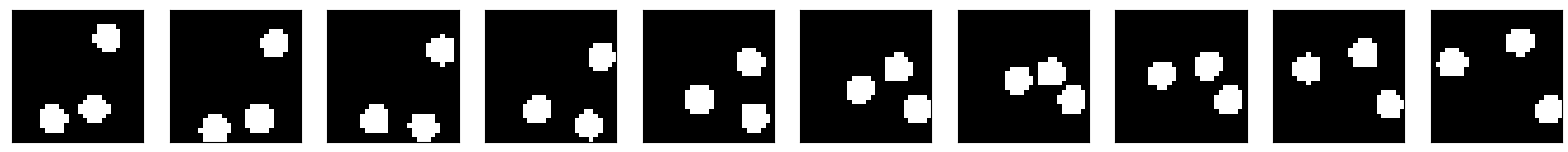
\includegraphics[scale=0.28]{Bilder/bouncingBalls}
    \end{figure}
\end{frame}




\begin{frame}
\frametitle{Ergebnisse}
\textbf{Von links nach rechts:} Modellinput, tatsächlicher Verlauf der \emph{time series}, Rekonstruktionen 
\begin{figure}[h!]
	\begin{minipage}{0.135\textwidth}
		%\begin{mdframed}[style=innersmall]
			\center{}
			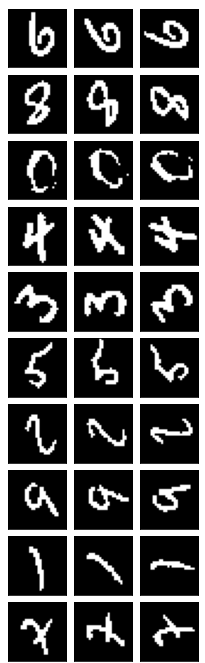
\includegraphics[scale=0.19]{Bilder/MNISTorig1}
			%\center{}
			%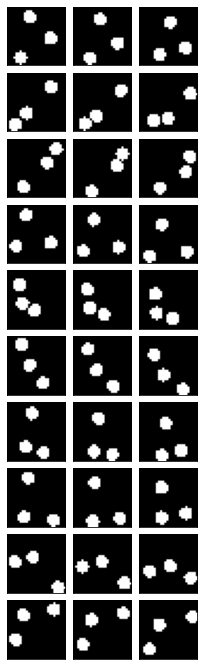
\includegraphics[scale=0.15]{Bilder/bouncingBalls_ODEorig1}
		%\end{mdframed}
	\end{minipage}
	\begin{minipage}{0.33\textwidth}
		%\begin{mdframed}[style=innersmall]
			\center{}
			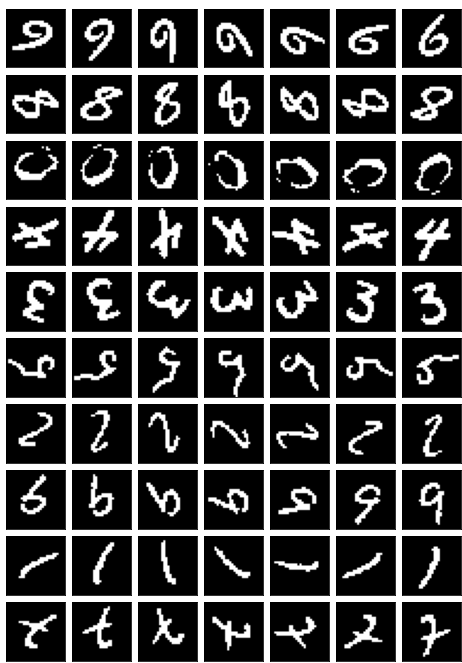
\includegraphics[scale=0.19]{Bilder/MNISTorig2}
			%\center{}
			%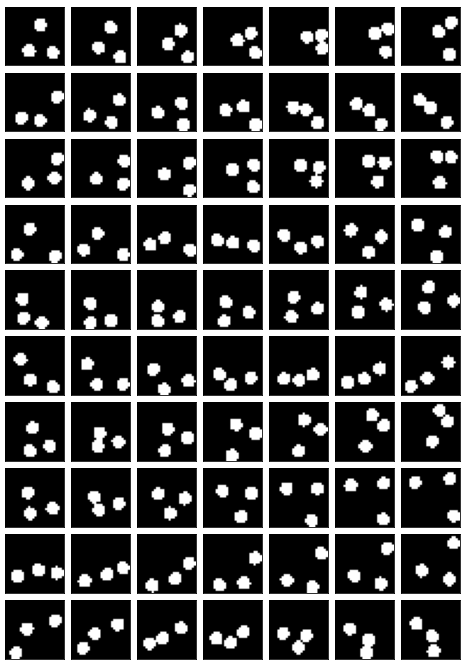
\includegraphics[scale=0.15]{Bilder/bouncingBalls_ODEorig2}
		%\end{mdframed}
	\end{minipage}
	\begin{minipage}{0.33\textwidth}
		%\begin{mdframed}[style=innersmall]
			\center{}
			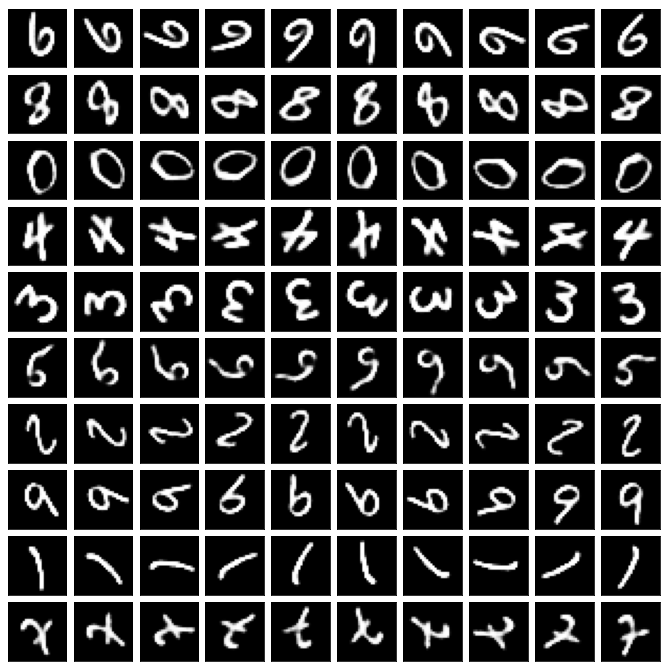
\includegraphics[scale=0.19]{Bilder/MNISTrec}
			%\center{}
			%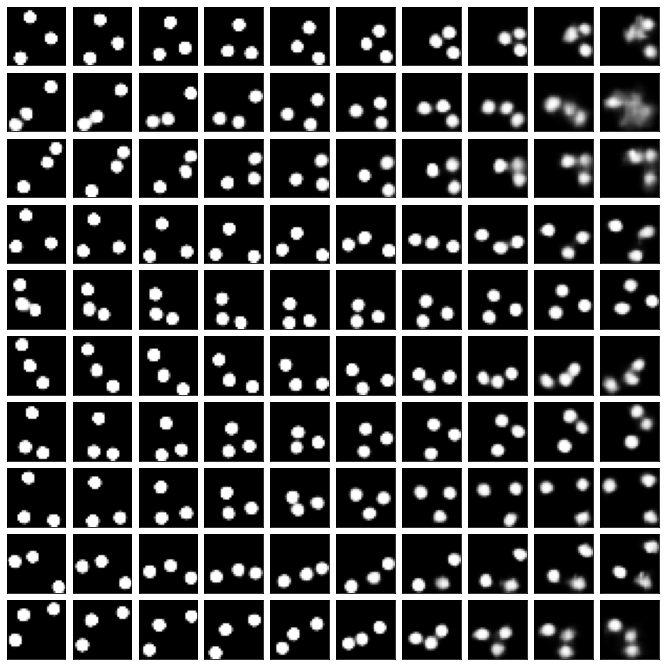
\includegraphics[scale=0.15]{Bilder/bouncingBalls_ODE}
		%\end{mdframed}
	\end{minipage}
\end{figure}
\end{frame}




\begin{frame}
\frametitle{Ergebnisse}
\textbf{Von links nach rechts:} Modellinput, tatsächlicher Verlauf der \emph{time series}, Rekonstruktionen 
\begin{figure}[h!]
	\begin{minipage}{0.135\textwidth}
		%\begin{mdframed}[style=innersmall]
		%\center{\small{Modellinput}\vspace{0.1cm}}
		%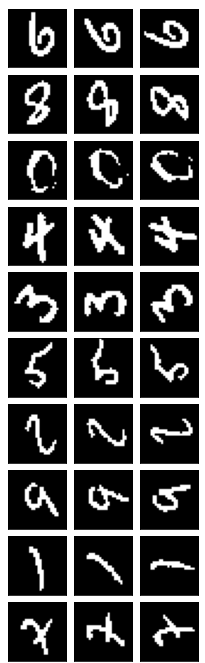
\includegraphics[scale=0.15]{Bilder/MNISTorig1}
		\center{}
		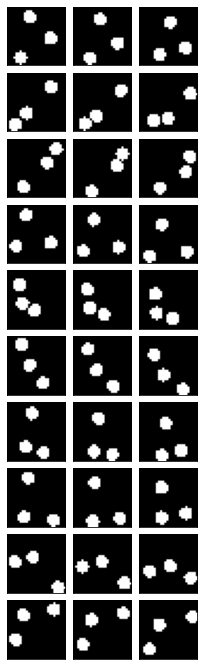
\includegraphics[scale=0.19]{Bilder/bouncingBalls_ODEorig1}
		%\end{mdframed}
	\end{minipage}
	\begin{minipage}{0.33\textwidth}
		%\begin{mdframed}[style=innersmall]
		%\center{Groundtruth\vspace{0.1cm}}
		%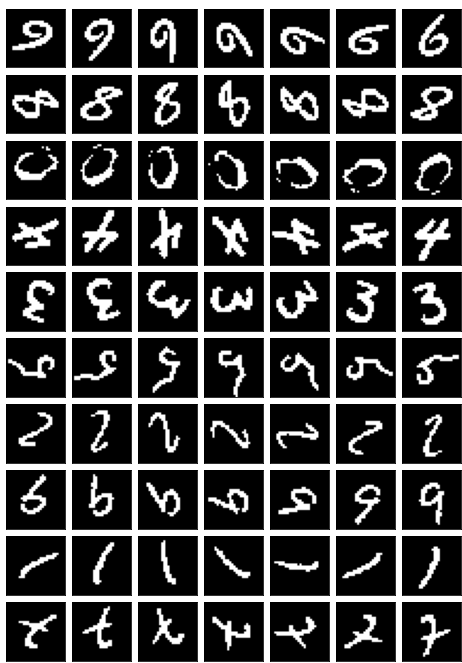
\includegraphics[scale=0.15]{Bilder/MNISTorig2}
		\center{}
		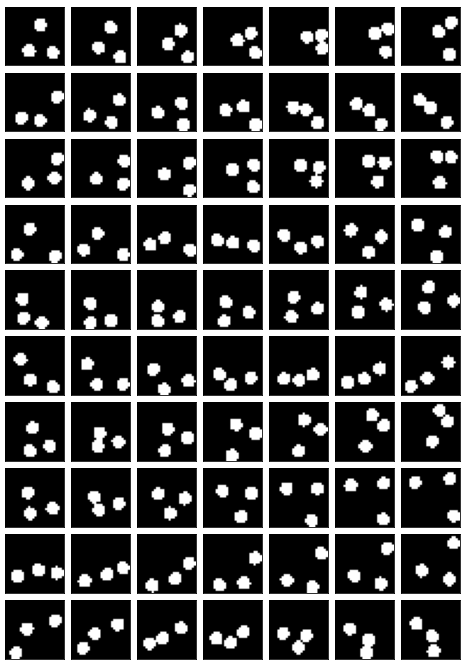
\includegraphics[scale=0.19]{Bilder/bouncingBalls_ODEorig2}
		%\end{mdframed}
	\end{minipage}
	\begin{minipage}{0.33\textwidth}
		%\begin{mdframed}[style=innersmall]
		%\center{Rekonstruktion}
		%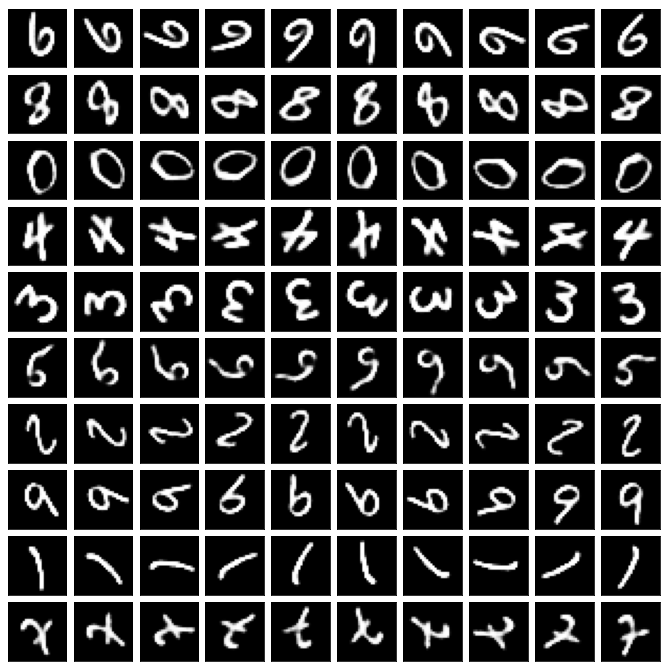
\includegraphics[scale=0.15]{Bilder/MNISTrec}
		\center{}
		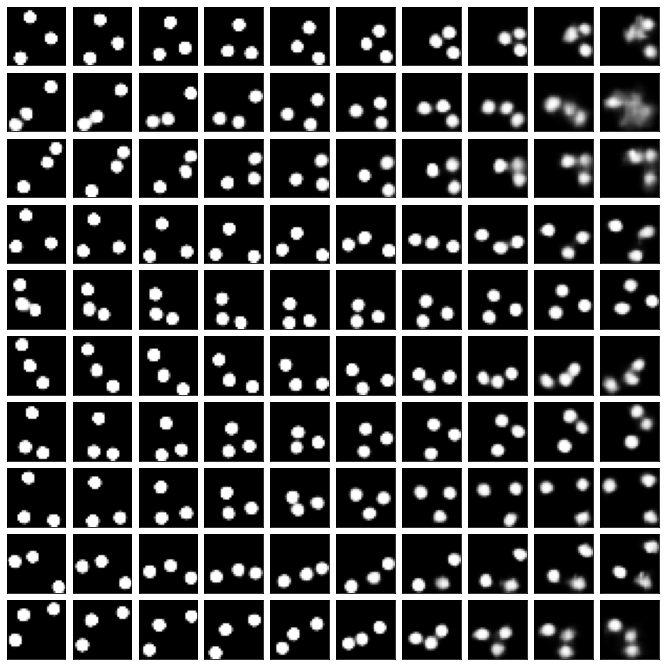
\includegraphics[scale=0.19]{Bilder/bouncingBalls_ODE}
		%\end{mdframed}
	\end{minipage}
\end{figure}
\end{frame}




%\begin{frame}
%\frametitle{Ergebnisse}
%\emph{AVI-Motion}
%\begin{figure}[!htbp]
%	\centering
%	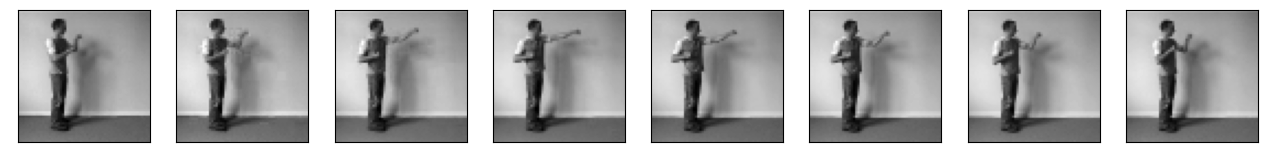
\includegraphics[scale=0.35]{Bilder/AVIMotion}
%\end{figure}
%\end{frame}




\begin{frame}
\frametitle{Ergebnisse}
\begin{figure}[h!]
	\begin{minipage}[position=l]{0.5\textwidth}
		%\begin{mdframed}[style=inner]
			\center{Modellinput\vspace{0.1cm}}
			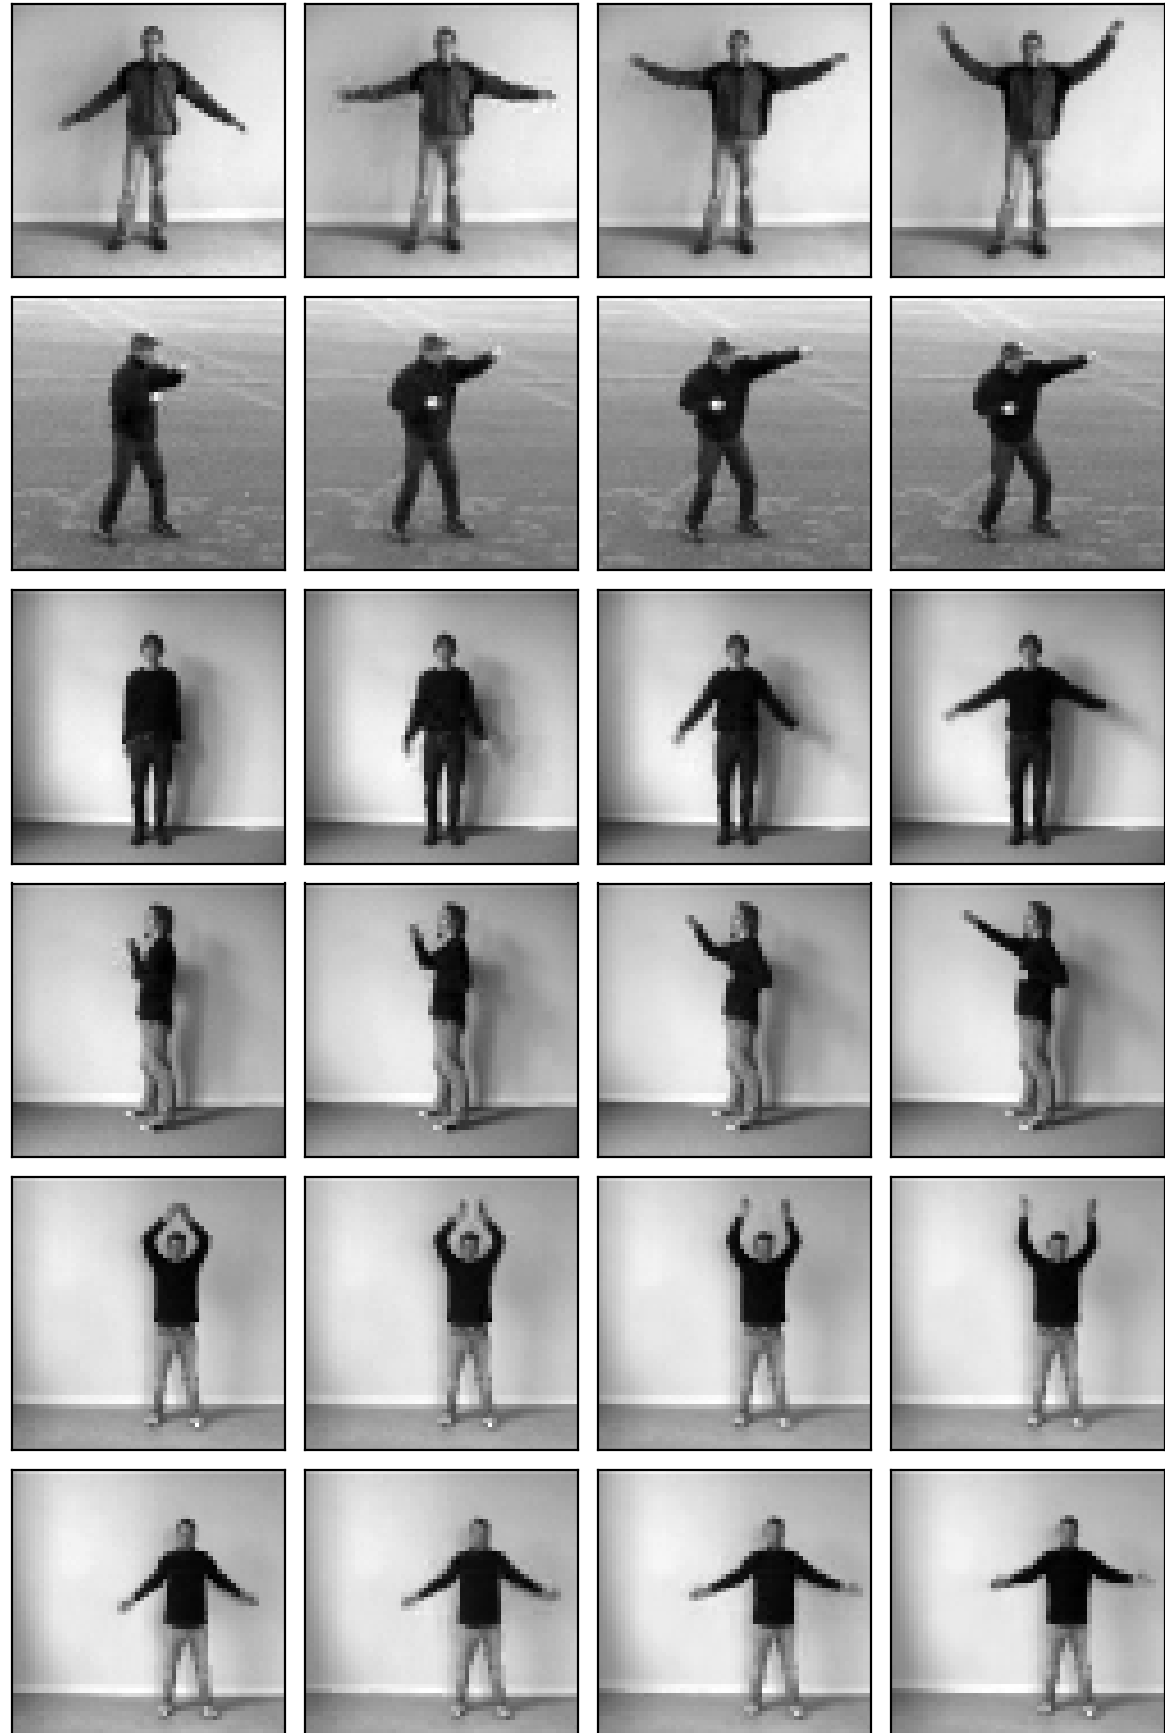
\includegraphics[scale=0.3]{Bilder/movies_input}
		%\end{mdframed}
	\end{minipage}
	\begin{minipage}[position=r]{0.4\textwidth}
		%\begin{mdframed}[style=inner]
			\center{Extrapolation\vspace{0.1cm}}
			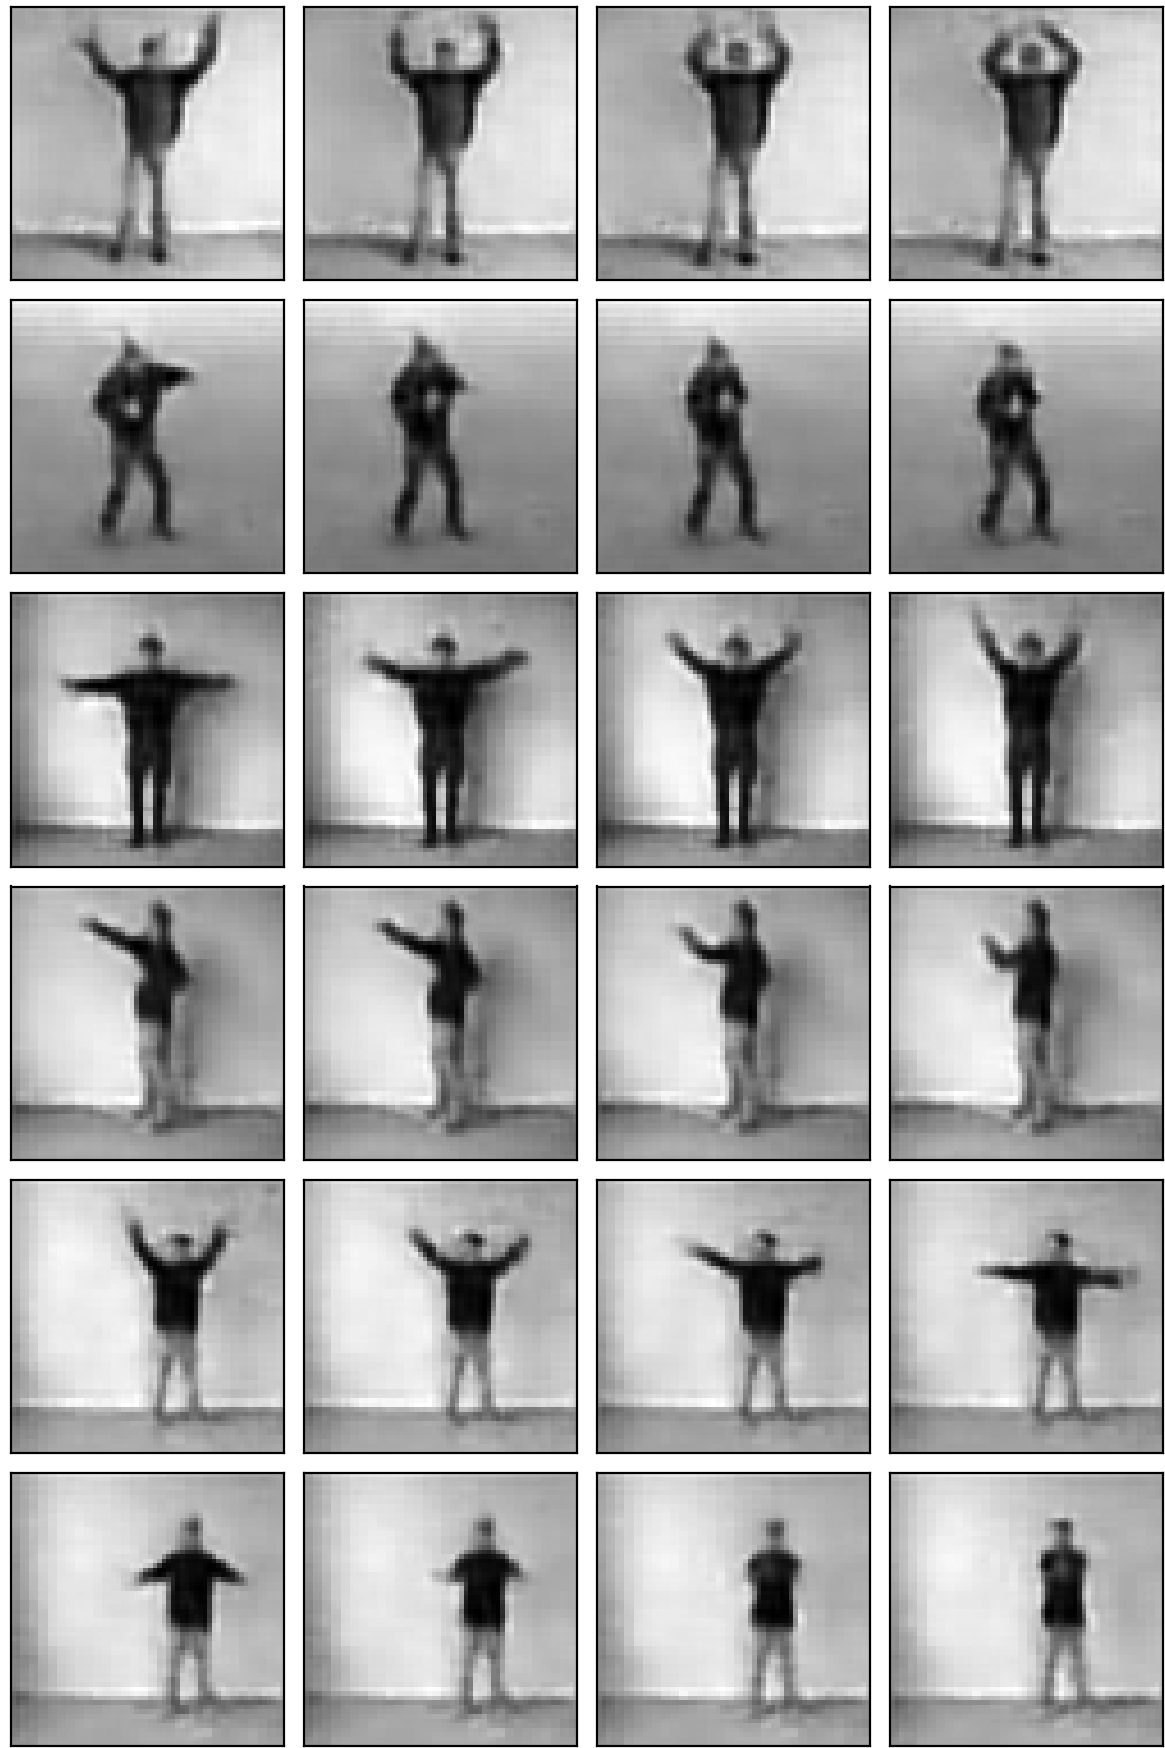
\includegraphics[scale=0.298]{Bilder/movies_extrapolation}
		%\end{mdframed}
	\end{minipage}
\end{figure}
\end{frame}

